\documentclass[a5paper,10pt]{article}
\usepackage[left=1cm,right=1cm,top=1.5cm,bottom=1cm]{geometry}

\usepackage{amsmath, amssymb}
\usepackage{mathtools}
\usepackage{titling}
\usepackage{fancyhdr}
\usepackage{enumitem}
\usepackage{cancel}
\usepackage{nicefrac}
\usepackage{bm}
\usepackage[svgnames]{xcolor}
\usepackage[b]{esvect}
\usepackage{tikz}
\usetikzlibrary{calc}
\usetikzlibrary {arrows.meta}
\usetikzlibrary{patterns}
\usepackage{tkz-euclide}
\usepackage[small]{titlesec}% Change sections font size

\usepackage[T1]{fontenc}
\usepackage{libertine}

% Document setup
\newcommand{\assignmentauthor}{github/3fxcf9}
\newcommand{\assignmentdate}{Baccalaureat 2024}
\newcommand{\assignmenttitle}{Physique}

% Header and Footer setup
\pagestyle{fancy}
\fancyhf{}
\fancyhf[lh]{\assignmentauthor}
\fancyhf[ch]{\itshape\assignmenttitle}
\fancyhf[rh]{\assignmentdate}
\fancyhf[rf]{\thepage}

% Line spacing
\titlespacing*{\section}{0pt}{0.1\baselineskip}{0.2\baselineskip}
\titlespacing*{\subsection}{0pt}{0.1\baselineskip}{0.2\baselineskip}

% Usefull commands
\newcommand*{\N}{\mathbb{N}}
\newcommand*{\Z}{\mathbb{Z}}
\newcommand*{\R}{\mathbb{R}}
\renewcommand*{\P}{\mathbb{P}}
\renewcommand*{\vec}{\vv}

\begin{document}
\renewcommand{\headsep}{10pt}
\thispagestyle{empty}
\vspace*{-1cm}
\noindent\assignmentauthor \hfill \assignmentdate
\vspace{-6pt}
\begin{center}
    \rule[2ex]{\textwidth}{1pt}\\
    \vspace{-4pt}
    {\Large{\assignmenttitle}}
    \vspace{-4pt}
\end{center}
\rule[2ex]{\textwidth}{1pt}\\
\title{}
\author{}
\date{}
\vspace{-0.5cm}
\section{Dynamique}
\subsection{Rappels: Théorème de l'énergie mécanique/cinétique}
\[
	\Delta E_c = \sum W(\vec{F}) \quad\text{ et }\quad \Delta E_m = \sum W(\vec{F_{NC}})
\]
\subsection{Rappels: Mouvement dans un champ uniforme}
\[
  \vec{P}=m\vec{g}\;;\  W_{\!\!AB}(\vec{P})=mg(z_A-z_B) \quad\mid\quad \vec{Fe}=q\vec{E}\;;\  W_{\!\!AB}(\vec{Fe})=q\cdot U_{\!\!AB}
\]

\subsection{Loi de Newton}
$$\sum{F_{ext}}=m\cdot\vec{a}$$

\subsection{Principe général}
Dans un repère $(O, \vec{u_1}, \vec{u_2})$, l'objet étudié est modélisé par le point $M$.
$$\hspace{-2em}\vec{a}=\frac{d\vec{v}}{dt}=\frac{d^2\vec{OM}}{dt^2}$$
\subsection{Mouvement circulaire}
\begin{minipage}[t]{0.55\linewidth}
    Dans la base de Frenet $(O,\vec{u_T},\vec{u_N})$,
  $\displaystyle \vec{a}\left(\frac{dv}{dt};\frac{v^2}{r}\right)$:\\[4pt]
    $\displaystyle \vec{a}=\frac{d\vec{v}}{dt}=\frac{d(v\vec{u_T})}{dt}=\frac{dv}{dt}\vec{u_T}+\frac{v^2}{r}\vec{u_N}$
    \begin{itemize}[noitemsep]
        \item $\vec{a_T}$ est l'accélération \textbf{tangentielle}.
        \item $\vec{a_N}$ est l'accélération \textbf{centripète}.
    \end{itemize}
\end{minipage}
\begin{minipage}[t]{0.4\linewidth}
    \vspace*{-2cm}
    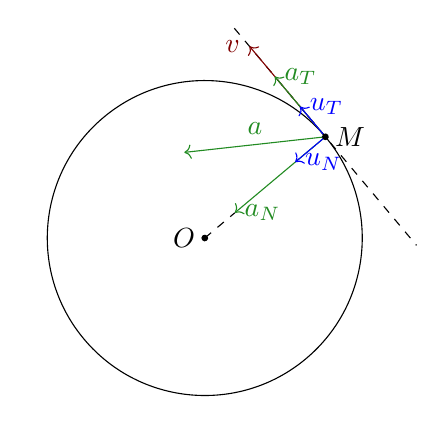
\begin{tikzpicture}[baseline=(current bounding box.north),rotate=40]
        % Define radius
        \def\r{2}
        \coordinate (o) at (0, 0);% Origin
        \coordinate (m) at (\r, 0);% Point on circle

        % Circle
        \filldraw (o) circle(1pt) node[left]{$O$};
        \draw (o) circle (\r);
        \draw[dashed] (o) -- (0.5, 0);
        \draw[dashed] (\r, 1.8) -- (\r, -1.8);

        % Velocity vector
        \draw[->, Maroon] (m) -- ++(0, 1.5) node[left] {$\vec{v}$};

        % Acceleration vectors
        \draw[->, ForestGreen] (m) -- ++(-1.5, 0) node[right] {$\vec{a_N}$};
        \draw[->, ForestGreen] (m) -- ++(0, 1) node[right] {$\vec{a_T}$};
        \draw[->, ForestGreen] (m) -- ++(-1.5, 1) node[midway,above]{$\vec{a}$};

        % Frenet base
        \draw[->, blue] (m) -- ++(-0.5, 0) node[right] {$\vec{u_N}$};
        \draw[->, blue] (m) -- ++(0, 0.5) node[right] {$\vec{u_T}$};
        \filldraw (m) circle(1pt) node[right]{$M$};
    \end{tikzpicture}
\end{minipage}

\subsection{Satellites}
La force d'attraction gravitationnelle entre deux corps de masse $m_A$ et $m_B$ se note:
$$\vec{F_G}=G\frac{m_Am_B}{r^2}\vec{u_N} \quad \text{ avec } \quad G\approx 6.67\cdot 10^{-11}N\cdot m^{2}\cdot kg^{-2}$$
Si $\sum{\vec{F_{ext}}}=\vec{F_G}$, pour un satellite de masse $m$ en orbite autour d'un corps de masse $M$:
$$\sum{\vec{F_{ext}}}=m\vec{a_N}=G\frac{m\times M}{r^2}\vec{u_N} \iff \vec{a_N}=\frac{GM}{r^2}$$
Nous savons que $\vec{a_N}=\frac{v^2}{r}$, ce qui nous donne:
$$\frac{v^2}{r}=\frac{GM}{r^2} \iff v=\sqrt{\frac{GM}{r}}$$
Nous pouvons alors calculer la période de rotation $T$ du satellite:
\begin{equation}\label{eq:1} T=\frac{2\pi r}{v}=2\pi\frac{\sqrt{r^2}}{v}=2\pi\sqrt{r^2\times\frac{r}{GM}}=2\pi\sqrt{\frac{r^3}{GM}}\end{equation}
\subsection{Lois de Kepler}
\begin{minipage}[t]{0.55\linewidth}
    \begin{enumerate}
        \item Les planètes du système solaire décrivent des trajectoires elliptiques, dont le Soleil\linebreak occupe un des foyers.
        \item Des aires égales sont balayées dans des temps égaux (aires grises ci-contre).
        \item $\displaystyle \frac{T^2}{r^3}=\frac{4\pi^2}{GM}=cte$ \qquad (à partir de (\ref{eq:1}))
    \end{enumerate}
\end{minipage}
\begin{minipage}[t]{0.4\linewidth}
    \vspace*{-1cm}
    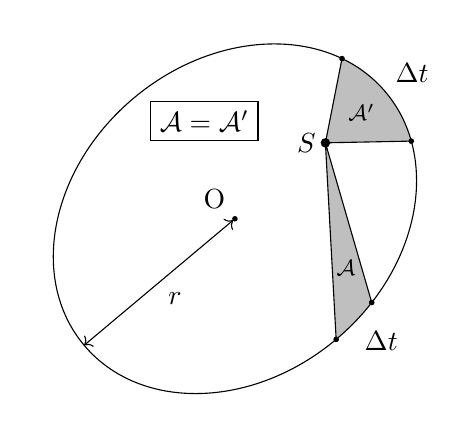
\begin{tikzpicture}[dot/.style={draw,fill,circle,inner sep=1pt},rotate=40]
        \def\a{2.5} % large half axis
        \def\b{2} % small half axis

        % Draw the ellipse
        \def\orbit{(0,0) ellipse ({\a} and {\b})}

        % Center
        \fill (0,0) coordinate (O) circle (1pt) node[above left] {O};

        % Nodes at the focal points
        \coordinate (S) at ({+sqrt(\a*\a-\b*\b)},0);

        % Demi grand axe
        \coordinate (axe) at (180:{\a} and {\b}) {};
        \draw[<->] ($(O)-(0.03,0)$) -- (axe) node[midway, below right] {$r$};

        % Points
        \coordinate (A1) at (20:{\a} and {\b});
        \coordinate (A2) at (-20:{\a} and {\b}) {};
        \coordinate (B1) at (-75:{\a} and {\b}) {};
        \coordinate (B2) at (-90:{\a} and {\b}) {};

        \begin{scope}  % The blue shaded regions
            \clip \orbit;
            \filldraw[fill=lightgray,rounded corners=.1pt] (S) -- ($2*(A1)-(S)$) -- ($2*(A2)-(S)$) -- cycle;
            \filldraw[fill=lightgray,rounded corners=.1pt] (S) -- ($2*(B1)-(S)$) -- ($2*(B2)-(S)$) -- cycle;
        \end{scope}

        % Delta T
        \draw[] (0:{\a} and {\b}) node[above right]{$\Delta t$};
        \draw[] (-82.5:{\a} and {\b}) node[below right]{$\Delta t$};

        \coordinate (L1) at ($(0:{\a} and {\b})-(S)$);
        \coordinate (L2) at ($(-82.5:{\a} and {\b})-(S)$);
        \draw[] ($(S)+0.6*(L1)$) node[]{\footnotesize $\mathcal{A}'$};
        \draw[] ($(S)+0.7*(L2)$) node[]{\footnotesize $\mathcal{A}$};
        \node[draw] at (0.5,1.2) {$\mathcal{A}=\mathcal{A}'$};

        \draw \orbit;

        \filldraw (A1) circle(.8pt);
        \filldraw (A2) circle(.8pt);
        \filldraw (B1) circle(.8pt);
        \filldraw (B2) circle(.8pt);

        \filldraw (S) circle(1.5pt) node[left]{$S$};
    \end{tikzpicture}
\end{minipage}
\vspace*{-8pt}

\section{Thermodynamique}
\subsection{Système thermodynamique}
\begin{itemize}[noitemsep]
    \item \textbf{Système ouvert}: Échange de matière et d'énergie avec l'extérieur.
    \item \textbf{Système fermé}: Échange d'énergie uniquement.
    \item \textbf{Système isolé}: Aucun échange avec l'extérieur.
\end{itemize}
\subsection{Modèle du gaz parfait}
Pour un gaz parfait (gaz dont les molécules n'interagissent que lors de chocs et dont la taille est insignifiante face à la distance intermoléculaire moyenne):
$$PV=nRT \quad\text{ avec }\quad R\approx8.31 \,J\cdot K^{-1}\cdot mol^{-1}$$
\subsection{Energie interne}
L'énergie totale d'un système $E_\text{globale}$ se note:
$$E_\text{globale} =  E_\text{cin,macro}  +  E_\text{pot,macro} + U$$
où $U$ est l'énergie interne. Si le système est au repos à l'échelle macroscopique:
$$\Delta E_\text{globale} = \Delta U = W+Q$$
\subsection{Systèmes incompressibles ($\rho$ constante)}
$$\Delta U = mc\Delta T \quad \text{où $c$ represente la \textit{capacité thermique massique}}$$
\subsection{Transferts thermiques}
Trois modes de transferts: \textbf{conduction} (de proche en proche) / \textbf{convection} (transferts induits par les mouvements d'un fluide) / \textbf{rayonnement} (rayonnement electromagnétique).\\[4pt]
Le flux thermique (chaleur) $\phi$ d'un corps de temp. $T_1$ à un corps de temp. $T_2$ s'exprime:
$$\phi = \frac{Q}{\Delta t} = \frac{T_1-T_2}{R_{\text{th}}} \quad \text{avec $R_{\text{th}}$ la résistance thermique de la paroi}$$
\subsection{Loi de Newton}


Elle décrit le transferts thermique entre un système \textbf{incompressible} de température $T$ et une \textbf{paroi thermostatée} de température $T_e$.
    {\setlength{\abovedisplayskip}{3pt}\setlength{\belowdisplayskip}{3pt}$$\phi = hS(T_e-T)$$}
    {\footnotesize Pour établir l'éq. diff: Supp. $W=0 \Rightarrow Q=mc\Delta T$ et $Q=\phi\Delta t=hS(T_e-T)\Delta t$ puis diviser par $mc$ et $\Delta t$\pagebreak}

\section{Bilan ratiatif terrestre}
\subsection{Loi de Stefan-Boltzmann}
La puissance surfacique $p$ émise par un corps noir (réémet tout rayonnement qu'il absorbe):
$$p=\sigma T^4 \quad \text{ avec } \quad\sigma=5,67\cdot 10^{-8}W.m^{-2}.K^{-4}$$
\begin{minipage}[t]{0.55\linewidth}
    La température sur terre est constante:
    $$\begin{aligned}
            \Delta U=\cancel{W}+Q =                  & Q_T+Q_R+Q_E          & = 0 \\
            \text{\footnotesize$(\div\Delta t)$}\iff & \phi_T+\phi_R+\phi_E & = 0 \\
            \text{\footnotesize$(\div S)$}\iff       & p_T+p_R+p_E          & = 0
        \end{aligned}$$
\end{minipage}
\begin{minipage}[t]{0.4\linewidth}
    \vspace*{0pt}
    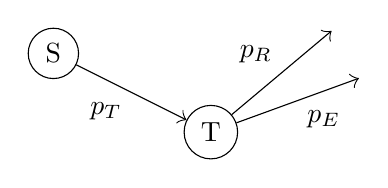
\begin{tikzpicture}
        \node[circle, draw=black] (S) at (-2, 1) {S};
        \node[circle, draw=black] (T) at (0, 0) {T};

        \draw[-{Classical TikZ Rightarrow[length=1mm]}] (S) -- (T) node[midway, below left] {$p_T$};
        \draw[-{Classical TikZ Rightarrow[length=1mm]}] (T) -- (40:2) node[midway, above left] {$p_R$};
        \draw[-{Classical TikZ Rightarrow[length=1mm]}] (T) -- (20:2) node[midway, below right] {$p_E$};
    \end{tikzpicture}
\end{minipage}
\\[6pt]La terre étant un corps noir:
$$-p_E=\sigma T_T^4 \implies T_T=\sqrt[4]{\frac{-p_E}{\sigma}}=\sqrt[4]{\frac{p_T+p_R}{\sigma}}$$
\subsection{L'albédo}
$$\alpha=\left\lvert\frac{p_R}{p_T}\right\rvert$$

\section{Diffraction et interférences}
\subsection{Diffraction}
C'est le changement de direction de propagation d'une onde à l'encontre d'une ouverture de l'ordre de sa longueur d'onde (ou plus dans le cas d'ondes électromagnétiques).
\begin{minipage}[t]{0.55\linewidth}
    \vspace*{0pt}
    L'angle caractéristique $\theta$ (angle du rayon passant par la première zone d'extinction) s'écrit:
    $$tan\theta = \frac{L}{2D} \approx \theta \quad \text{ car } \theta \text{ petit}$$
    Et aussi (Le coefficient $1.22$ est spécifique aux ouvertures circulaires):
    $$sin\theta = 1.22 \times \frac{\lambda}{a}\approx\theta \quad \text{ car } \theta \text{ petit}$$
\end{minipage}
\begin{minipage}[t]{0.05\linewidth}
    \phantom{a}
\end{minipage}
\begin{minipage}[t]{0.4\linewidth}
    \vspace*{0pt}
    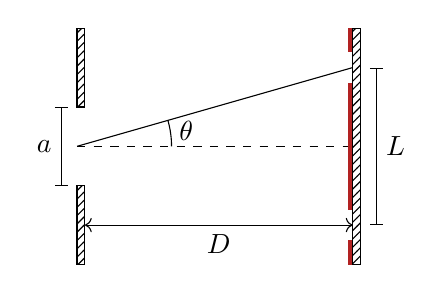
\begin{tikzpicture}
        \def\a{-1.5}
        \def\b{2}
        \def\aa{-1.7}

        \draw[dashed] (\a,0) -- (\b,0);

        \draw[pattern=north east lines] (\a,-1.5) rectangle ++(0.1,1);
        \draw[pattern=north east lines] (\a,1.5) rectangle ++(0.1,-1);
        \draw[fill=FireBrick, draw=FireBrick] ($(\b,-0.8)-(0.05,0)$) rectangle ++(0.05,1.6);
        \draw[fill=FireBrick, draw=FireBrick] ($(\b,-1.2)-(0.05,0)$) rectangle ++(0.05,-0.3);
        \draw[fill=FireBrick, draw=FireBrick] ($(\b,1.2)-(0.05,0)$) rectangle ++(0.05,0.3);
        \draw[pattern=north east lines] (\b,-1.5) rectangle ++(0.1,3);


        \coordinate (X) at (\a,0);
        \coordinate (Y) at (\b,1);
        \coordinate (Z) at (\b,0);

        \draw (X) -- (Y);

        \draw[|-|] (\aa,0.5) -- (\aa,-0.5) node [midway, left] {$a$};
        \draw[|-|] (2.3,1) -- (2.3,-1) node [midway, right] {$L$};
        \draw[<->] ($(\a,-1)+(0.1,0)$) -- (\b,-1) node [midway, below] {$D$};


        \tkzMarkAngle[size=1.2cm](Z,X,Y)
        \tkzLabelAngle[pos=1.4](Z,X,Y){$\theta$}
    \end{tikzpicture}
\end{minipage}
\subsection{Interférences}
\begin{minipage}[t]{0.55\linewidth}
    \vspace*{0pt}
    \begin{itemize}[noitemsep]
        \item \textbf{Constructives}: $\delta=k\lambda, k\in\Z$
        \item \textbf{Destructives}: $\delta=(2k+1)\frac{\lambda}{2}, k\in\Z$
    \end{itemize}
    Dans le dispositif des \textbf{fentes d'Young}, la différence de marche $\delta$ en un point d'abscisse $x$:
    $$\delta=\frac{bx}{D}$$
\end{minipage}
\begin{minipage}[t]{0.05\linewidth}
    \phantom{a}
\end{minipage}
\begin{minipage}[t]{0.4\linewidth}
    \vspace*{0pt}
    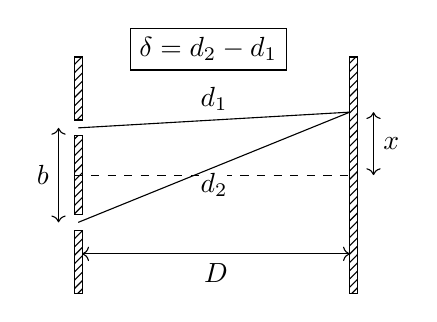
\begin{tikzpicture}
        \def\a{-1.5}
        \def\b{2}
        \def\aa{-1.7}
        \def\aaa{-1.45}
        \def\bb{2.3}

        \draw[dashed] (\a,0) -- (\b,0);

        \draw[pattern=north east lines] (\a,-1.5) rectangle ++(0.1,0.8);
        \draw[pattern=north east lines] (\a,1.5) rectangle ++(0.1,-0.8);
        \draw[pattern=north east lines] (\a,0.5) rectangle ++(0.1,-1);
        \draw[pattern=north east lines] (\b,-1.5) rectangle ++(0.1,3);

        \coordinate (X) at (\b,0.8);

        \draw (\aaa,0.6) -- (X) node [midway, above] {$d_1$};
        \draw (\aaa,-0.6) -- (X) node [midway, below=2pt, fill=white, inner sep=0pt] {$d_2$};

        \draw[<->] (\aa,0.6) -- (\aa,-0.6) node [midway, left] {$b$};
        \draw[<->] (\bb,0.8) -- (\bb,0) node [midway, right] {$x$};
        \draw[<->] ($(\a,-1)+(0.1,0)$) -- (\b,-1) node [midway, below] {$D$};

        \node[draw] at (0.2,1.6) {$\delta=d_2-d_1$};
    \end{tikzpicture}
\end{minipage}
\subsection{Interfrange}
On peut alors calculer l'interfrange $i$, distance entre deux franges brillantes ou sombres consécutives:
$$
i=x_{k+1}-x_k=\frac{(k+1)\lambda D}{b}-\frac{k\lambda D}{b}=\frac{\lambda D}{b}
$$

\section{Dynamique du dipôle RC}
\textbf{Loi des nœuds}: La somme des intensités des courants qui entrent par un nœud est égale à la somme des intensités des courants qui sortent du même nœud.\\
\textbf{Loi des mailles}: La somme algébrique des différences de potentiel le long d'une maille est constamment nulle.\\
\textbf{Loi d'Ohm}: $U=Ri$
\subsection{Capacité}
La capacité $C$ en Farads d'un condensateur dont $q$ est la charge de la borne positive s'écrit:
$$C=\frac{q}{U_c} \iff q=CU_c$$
\subsection{L'intensité électrique}
Elle correspond au débit des changes électriques:
$$i=\frac{dq}{dt}\;(=)\;C\frac{dU_c}{dt}$$
\subsection{Temps caractéristique}
Le temps caractéristique $\tau$ est le temps nécessaire pour charger un condensateur à $63\%$ de sa capacité\footnote{Pour établir l'équation différentielle: Loi des mailles, puis d'Ohm, puis réécrire l'intensité}
. On le note:
$$\tau=RC$$

\section{Lunette astronomique}
\begin{minipage}[t]{0.55\linewidth}
    \vspace*{0pt}
    \subsection{Lentille mince convergente}
    $\bm{\Delta}$: Axe optique ; \quad $\bm{O}$: Centre optique\\
    $\bm{AB}$: Objet ; \quad $\bm{A'B'}$: Image\\
    $\bm{F}$ (resp. $\bm{F'}$): Foyer objet (resp. image)\\
    $\bm{f}$ (resp. $\bm{f'}$): Distance focale objet (resp. image)\\
    $\bm{P_{f,i}}$ (resp. $\bm{P_{f,o}}$): Plan focal image (resp. objet)
\end{minipage}
\begin{minipage}[t]{0.05\linewidth}
    \phantom{a}
\end{minipage}
\begin{minipage}[t]{0.4\linewidth}
    \vspace*{-10pt}
    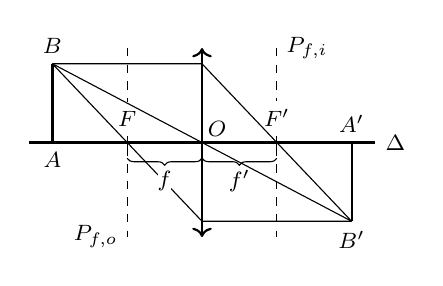
\begin{tikzpicture}
        \def\a{-2.2}
        \def\b{2.2}
        \def\o{0}
        \def\i{-1.9}
        \def\h{1}
        \def\f{0.5*\i}

        \draw[thick] (\a,0) -- (\b,0) node [right] {\footnotesize $\Delta$};

        \draw[<->, thick] (\o,\h+0.2) -- (\o,-\h-0.2);
        \node[above right=-2pt] (\o,0) {\footnotesize $O$};

        % Dashed lines
        \draw[dashed] (-\f,\h+0.2) node[right] {\footnotesize $P_{f,i}$} -- (-\f,-\h-0.2);
        \draw[dashed] (\f,\h+0.2) -- (\f,-\h-0.2) node[left] {\footnotesize $P_{f,o}$};

        % Foyers
        \draw (\f, 0.1) -- (\f, -0.1) node [above=5pt, fill=white] {\footnotesize $F$};
        \draw (-\f, 0.1) -- (-\f, -0.1) node [above=5pt, fill=white] {\footnotesize $F'$};
        
        % Object
        \draw[thick] (\i, 0) node[below] {\footnotesize $A$} -- (\i, \h) node[above] {\footnotesize $B$};
        \draw[thick] (-\i, 0) node[above] {\footnotesize $A'$} -- (-\i, -\h) node[below] {\footnotesize $B'$};

        % Rays
        \draw (\i, \h) -- (-\i, -\h);
        \draw (\i, \h) -- (\o, \h) -- (-\i,-\h);
        \draw (\i, \h) -- (\o, -\h) -- (-\i,-\h);


        \draw [
                decoration={
                        brace,
                        raise=0.2cm
                    },
                decorate
              ] (\o, 0) -- (\f, 0) node[below=10pt, midway, align=center, fill=white, inner sep=0pt] {\footnotesize $f$};
        \draw [
                decoration={
                        brace,
                        raise=0.2cm
                    },
                decorate
              ] (-\f, 0) -- (\o, 0) node[below=10pt, midway, align=center, fill=white, inner sep=0pt] {\footnotesize $f'$};
    \end{tikzpicture}
\end{minipage}
\vspace{1em}
\begin{minipage}[t]{0.4\linewidth}
    \vspace*{1em}
    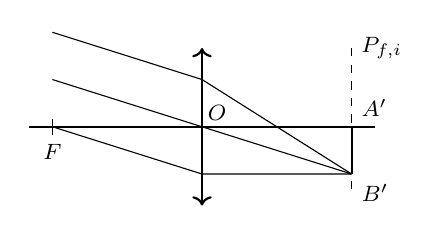
\begin{tikzpicture}
        \def\a{-2.2}
        \def\b{2.2}
        \def\o{0}
        \def\i{-1.9}
        \def\h{0.6}
        \def\f{\i}

        \draw[thick] (\a,0) -- (\b,0);

        \draw[<->, thick] (\o,\h+0.4) -- (\o,-\h-0.4);
        \node[above right=-2pt] (\o,0) {\footnotesize $O$};

        % Dashed lines
        \draw[dashed] (-\f,\h+0.4) node[right] {\footnotesize $P_{f,i}$} -- (-\f,-\h-0.2);

        % Foyers
        \draw (\f, 0.1) -- (\f, -0.1) node [below, fill=white] {\footnotesize $F$};
        
        % Object
        \draw[thick] (-\i, 0) node[above right] {\footnotesize $A'$} -- (-\i, -\h) node[below right] {\footnotesize $B'$};

        % Rays
        \draw (\i, \h) -- (-\i, -\h);
        \draw (-\f, -\h) -- (\o,\h) -- ++(\i,\h);
        \draw (\f, 0) -- (\o,-\h) -- (-\i,-\h);
    \end{tikzpicture}
\end{minipage}
\begin{minipage}[t]{0.05\linewidth}
    \phantom{a}
\end{minipage}
\begin{minipage}[t]{0.55\linewidth}
    \vspace*{1em}
    \subsection{Objet à l'infini / au foyer objet}
    L’image d'un objet situé à l'infini se forme sur le plan focal, et l'image d'un objet situé sur le plan focal se forme à l'infini.
\end{minipage}

\subsection{Composition d'une lunette astronomique}
    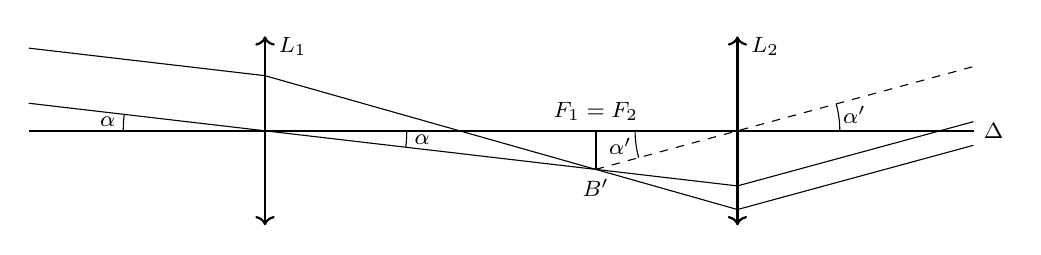
\begin{tikzpicture}
        \def\a{-3}
        \def\b{-\a}
        \def\h{1.2}
        \def\extraend{1.665}
        \def\extrabeg{0.5}

        \draw[thick] (-6,0) -- (6,0) node[right] {\footnotesize $\Delta$};
        \draw[<->, thick] (\a,\h) node[xshift=10pt, yshift=-3.5pt] {\footnotesize $L_1$} -- (\a,-\h);
        \draw[<->, thick] (\b,\h) node[xshift=10pt, yshift=-3.5pt] {\footnotesize $L_2$} -- (\b,-\h);

        % Rays
        \path (\a,0) -- (\b,-\h+0.5) coordinate[pos=-\extrabeg](binf);
        \draw (binf) -- (\a,0) -- (\b,-\h+0.5) -- ++(1.8*\extraend,0.49*\extraend);
        
        \draw (\a,\h-0.5) -- (\b,-\h+0.2) -- ++(1.8*\extraend,0.49*\extraend);;
        \draw (\a,\h-0.5) -- ++(\extrabeg*-6,\extrabeg*0.7);

        \draw[thick] (1.2,0) node[above] {\footnotesize $F_1=F_2$} -- (1.2,-0.49) node[below] {\footnotesize $B'$};

        \path (1.2,-0.49) -- (\b,0) coordinate[pos=1+\extraend](dotinf);
        \draw[dashed] (1.2,-0.49) -- (dotinf);

        \tkzDefPoint(\a,0){A}
        \tkzDefPoint(-6,0){B}
        \tkzMarkAngle[size=1.8cm](binf,A,B)
        \tkzLabelAngle[pos=2](binf,A,B) {\footnotesize $\alpha$}
        \tkzMarkAngle[size=-1.8cm](binf,A,B)
        \tkzLabelAngle[pos=-2](binf,A,B) {\footnotesize $\alpha$}

        \tkzDefPoint(\b,0){X}
        \tkzDefPoint(6,0){Y}
        \tkzMarkAngle[size=1.3cm](Y,X,dotinf)
        \tkzLabelAngle[pos=1.5](Y,X,dotinf) {\footnotesize $\alpha'$}
        \tkzMarkAngle[size=-1.3cm](Y,X,dotinf)
        \tkzLabelAngle[pos=-1.5](Y,X,dotinf) {\footnotesize $\alpha'$}
    \end{tikzpicture}\\
    Elle est constituée d'un \textbf{objectif} ($L_1$) et d'un \textbf{oculaire} ($L_2$). La lunette est dite \textbf{afocale} si $F_1=F_2$. Dans ce cas, l'image est formée à l'infini. On note le \textit{grossissement} de la lunette
    \[
	    G=\frac{\alpha'}{\alpha}=\frac{f_1}{f_2} \quad\text{ en supposant }\quad \tan\theta\approx\theta
    \]

    \section{Sons et effet Doppler}
    \subsection{Intensité sonore}
    \vspace{-2em}
    \[
	I=\frac{P}{S}
    \]
    \subsection{Niveau d'intensité sononre \normalfont{(Level)}}
    \[
	    L=10\cdot\log\left(\frac{I}{I_0}\right) \iff I=I_0\cdot 10^{\frac{1}{10}L}  \quad\text{ où }\quad I_0=1.0\cdot 10^{-12}W\cdot m^2
    \]
    Remarque: $\displaystyle I'=2I \implies L'=10\cdot \log\left(\frac{2I}{I_0}\right) = 10\cdot\log\left(\frac{I}{I_0}\right)+10\cdot\log(2) \approx L+3$
    
    \subsection{Attenuation : \normalfont{différence de niveaux sonores. Si on double la distance à la source,}}
    $r'=2r \implies S'=4\pi (2r)^2 = 4S \implies I'=\frac{I}{4} \implies L'=L-10\cdot\log(4) \approx L-6$

\vspace{4pt}
    \subsection{Effet Doppler}
    $\displaystyle \Delta f=f_R-f_E$ est positif quand E et R se rapproche et négatif si ils s'éloignent.\\
    Pour un émetteur se rapprochant à la vitesse $v$ d'un récepteur et émettant onde de longueur d'onde $\lambda$ et de période $T$, on peut déterminer la fréquence $f'=\nicefrac{c}{\lambda'}$ perçue par le recepteur:
    \[
      \lambda'=\lambda-vT \iff \frac{c}{f'}=\frac{c}{f}-vt=\frac{c-v}{f} \iff f'=f\frac{c}{c-v}=\frac{f}{1-\frac{v}{c}}
    \]
    
    

    \section{Description d'un fluide au repos / modélisation de l'écoulement}
    \subsection{Pression et force pressante}
    \[
      F=\frac{P}{S} \quad\text{ et à température constante, }\quad PV=nRT=\mathrm{cte}
    \]

    \subsection{Pression dans un fluide incompressible au repos: \normalfont{augmente avec la profondeur}}
    \[
      \Delta P=\rho g h \iff P+\rho g z = \mathrm{cte} \quad\text{ car }\quad h=\Delta z
    \]
    
  \subsection{Poussée d'archimède}
  Elle est due à la différence de pression du fluide environnant entre le point haut et bas du système. Elle est une force opposée au poids du fluide déplacé.
  \[
    \vec{F_P}=-\rho V \vec{g}
  \]
  \subsection{Écoulement d'un fluide}
  \textbf{Régime permanent indép. du temps (stationnaire):} Vitesse indépendante du temps.
  Le débit volumique, \textbf{constant en régime permanent} pour un fluide incompressible vaut
  \[
    D_V=\frac{V}{\Delta T}=\frac{Sl}{\Delta T}=Sv
  \]
  où $l$ est la distance parcourue par le fluide dans une section $S$ en un temps $\Delta T$.

\vspace{4pt}
  \subsection{Relation de Bernoulli}
  Pour un fluide incompressible, le long d'une ligne de courant,
  \[
    \begin{aligned}
      \Delta Em=W_{AB}(\vec{F})=P_AV_A-P_BV_B &\implies \frac{1}{2}mv^2+mgz+PV=\mathrm{cte}\\
      & \implies \underbrace{\frac{1}{2}\rho v^2}_{\mathclap{\text{Correction dynamique appliquée à 8.2}}}+\rho g z + P = \mathrm{cte}
    \end{aligned}
  \]
  \subsection{Effet Venturi}
  C'est une conséquence de la relation de Bernoulli: pour une conduite horizontale, lorsque la section diminue, la vitesse augmente et la pression diminue.\\
  
\section{La lumière, un flux de photons}
\subsection{Intéraction avec la matière}
Lorsqu'un atome émet ou absorbe un photon, son niveau d'énergie $E$ change:\\[1em]
\vspace{1em}
\phantom{easter egg}$\displaystyle \Delta E=|E_f-E_i|=E_{\text{photon}} = h\nu = h\frac{c}{\lambda} \hfill\text{ \footnotesize(relation de Planck-Einstein)}$\\
où $\nu$ est la fréquence du rayonnement associé au photon absorbé et $h$ la constante de Plank.

\vspace{4pt}
\subsection{Effet photoélectrique}
Quand un photon entre en collision avec un électron présent dans un métal, il lui transmet son énergie. Si celle-ci est suffisamment grande, l'électron est éjecté. L'énergie minimale pour arracher un électron est le \textbf{travail d'extraction}, noté $W_{\text{extraction}}$. Le surplus éventuel d'énergie fourni par le photon est convertie en énergie cinétique $Ec_{\text{max}}$. On a donc
\[
  E_{\text{photon}}=h\nu=W_{\text{extraction}}+\frac{1}{2}mv^2
\]
Cet effet est utilisé dans les cellules photoélectriques (photorésistances, cellules photovoltaïques...) où les photons sont captés, et dans les diodes électroluminescentes (DEL) où ils sont émis.

  
  


\end{document}
